\documentclass{beamer}
\usepackage[utf8]{inputenc}

\usetheme{Madrid}
\usecolortheme{default}
\usepackage{amsmath,amssymb,amsfonts,amsthm}
\usepackage{txfonts}
\usepackage{tkz-euclide}
\usepackage{listings}
\usepackage[T1]{fontenc}
\usepackage{adjustbox}
\usepackage{array}
\usepackage{tabularx}
\usepackage{gvv}
\usepackage{lmodern}
\usepackage{circuitikz}
\usepackage{tikz}
\usepackage{graphicx}

\setbeamertemplate{page number in head/foot}[totalframenumber]

\usepackage{tcolorbox}
\tcbuselibrary{minted,breakable,xparse,skins}

\definecolor{bg}{gray}{0.95}
\DeclareTCBListing{mintedbox}{O{}m!O{}}{%
  breakable=true,
  listing engine=minted,
  listing only,
  minted language=#2,
  minted style=default,
  minted options={%
    linenos,
    gobble=0,
    breaklines=true,
    breakafter=,,
    fontsize=\small,
    numbersep=8pt,
    #1},
  boxsep=0pt,
  left skip=0pt,
  right skip=0pt,
  left=25pt,
  right=0pt,
  top=3pt,
  bottom=3pt,
  arc=5pt,
  leftrule=0pt,
  rightrule=0pt,
  bottomrule=2pt,
  toprule=2pt,
  colback=bg,
  colframe=orange!70,
  enhanced,
  overlay={%
    \begin{tcbclipinterior}
    \fill[orange!20!white] (frame.south west) rectangle ([xshift=20pt]frame.north west);
    \end{tcbclipinterior}},
  #3,
}

\lstset{
    language=C,
    basicstyle=\ttfamily\small,
    keywordstyle=\color{blue},
    stringstyle=\color{orange},
    commentstyle=\color{green!60!black},
    numbers=left,
    numberstyle=\tiny\color{gray},
    breaklines=true,
    showstringspaces=false,
}

\title{1.11.16}
\author{AI25BTECH11014 - Suhas}

\begin{document}

\frame{\titlepage}

\begin{frame}{Question}
Find the area of a triangle having the points
\[
\vec{A} = \myvec{1 \\ 1 \\ 1}, \quad
\vec{B} = \myvec{1 \\ 2 \\ 3}, \quad
\vec{C} = \myvec{2 \\ 3 \\ 1}
\]
as its vertices.
\end{frame}

\begin{frame}{ Theoretical Solution}
Let the vertices of the triangle be:
\[
\vec{A} = \myvec{1 \\ 1 \\ 1}, \quad
\vec{B} = \myvec{1 \\ 2 \\ 3}, \quad
\vec{C} = \myvec{2 \\ 3 \\ 1}
\]

To compute the area of triangle \(ABC\), we use the formula:
\[
\text{Area} = \frac{1}{2} \left\| (\vec{B} - \vec{A}) \times (\vec{C} - \vec{A}) \right\|
\]

Compute the vectors:
\[
\vec{B} - \vec{A} = \myvec{0 \\ 1 \\ 2}, \quad
\vec{C} - \vec{A} = \myvec{1 \\ 2 \\ 0}
\]
\end{frame}

\begin{frame}{ Theoretical Solution }

Now compute the cross product:
\[
(\vec{B} - \vec{A}) \times (\vec{C} - \vec{A}) =
\myvec{
(1)(0) - (2)(2) \\
(2)(1) - (0)(0) \\
(0)(2) - (1)(1)
} =
\myvec{-4 \\ 2 \\ -1}
\]

Next, compute the magnitude of the cross product:
\[
\left\| \myvec{-4 \\ 2 \\ -1} \right\| =
\sqrt{(-4)^2 + 2^2 + (-1)^2} =
\sqrt{16 + 4 + 1} = \sqrt{21}
\]
\end{frame}


\begin{frame}{ Theoretical Solution }

Therefore, the area of triangle \(ABC\) is:
\[
\text{Area} = \frac{1}{2} \cdot \sqrt{21}
\]

\[
\boxed{\text{Area} = \frac{\sqrt{21}}{2}}
\]

\end{frame}







\begin{frame}[fragile]{C Code}
\begin{lstlisting}
#include <math.h>
float area() {
  float A[3] = {1,1,1}, B[3] = {1,2,3}, C[3] = {2,3,1};
  float U[3] = {B[0]-A[0],B[1]-A[1],B[2]-A[2]};
  float V[3] = {C[0]-A[0],C[1]-A[1],C[2]-A[2]};
  float CP[3] = {
    U[1]*V[2]-U[2]*V[1],
    U[2]*V[0]-U[0]*V[2],
    U[0]*V[1]-U[1]*V[0]
  };
  return 0.5 * sqrt(CP[0]*CP[0]+CP[1]*CP[1]+CP[2]*CP[2]);
}
\end{lstlisting}
\end{frame}


\begin{frame}[fragile]{C Code for .so File }
\begin{lstlisting}
#include <math.h>

float triangle_area(float* U, float* V) {
  float CP[3] = {
    U[1]*V[2] - U[2]*V[1],
    U[2]*V[0] - U[0]*V[2],
    U[0]*V[1] - U[1]*V[0]
  };

  float mag = sqrt(CP[0]*CP[0] + CP[1]*CP[1] + CP[2]*CP[2]);
  return 0.5 * mag;
}
\end{lstlisting}
\end{frame}


\begin{frame}[fragile]{Python Code Using .so }
\begin{lstlisting}[language=Python]
import ctypes
import numpy as np

lib = ctypes.CDLL('./libtriangle.so')
lib.triangle_area.argtypes = [ctypes.POINTER(ctypes.c_float),
                              ctypes.POINTER(ctypes.c_float)]
lib.triangle_area.restype = ctypes.c_float

U = np.array([0, 1, 2], dtype=np.float32)
V = np.array([1, 2, 0], dtype=np.float32)

area = lib.triangle_area(U.ctypes.data_as(ctypes.POINTER(ctypes.c_float)),
                         V.ctypes.data_as(ctypes.POINTER(ctypes.c_float)))
print(f"Area = {area}")
\end{lstlisting}
\end{frame}






\begin{frame}{Plot}
\begin{figure}[H]
    \centering
    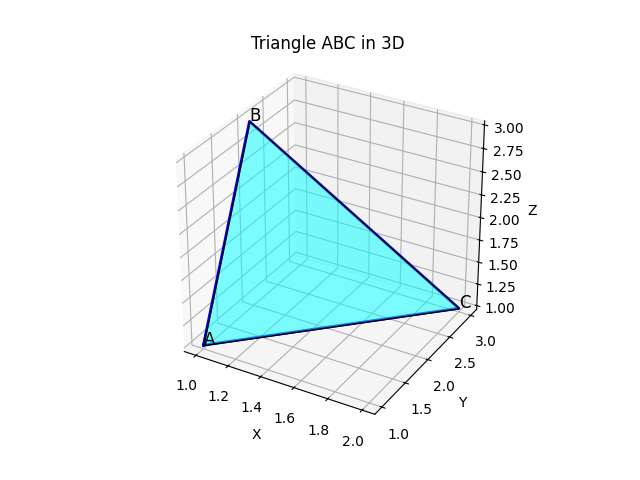
\includegraphics[width=0.78\linewidth]{Figs/fig1 (1).png}
    \caption{Triangle ABC}
    \label{fig:fig1}
\end{figure}
\end{frame}




\end{document}




